\section{Cel i zakres pracy}

Praca ta dokonuje analizy porównawczej trzech wybranych frameworków serwujących dane.
Pod uwagę został wzięty aspekt czasu odpowiedzi przy róznych warunkach.
Badanie ma na celu wzkazać mocne oraz słabsze strony każdego z porównywanych narzędzi.
Badany jest wycinek rzeczywistości, którego istoną częścią jest różnica.
Bezwględne wartości mogą się różnić w zależności od warunków uruchomienia, natomiast relacje między badanymi obiektami powinny być stale zauważalne.


Testy można dzielić na rodzaje pod różnymi względami. Podstawowy poział testów został zaprezentowny na rysynku \ref{rys:test-types}\cite{atlassianRneRodzaje}.
\begin{figure}[!hb]
	\centering 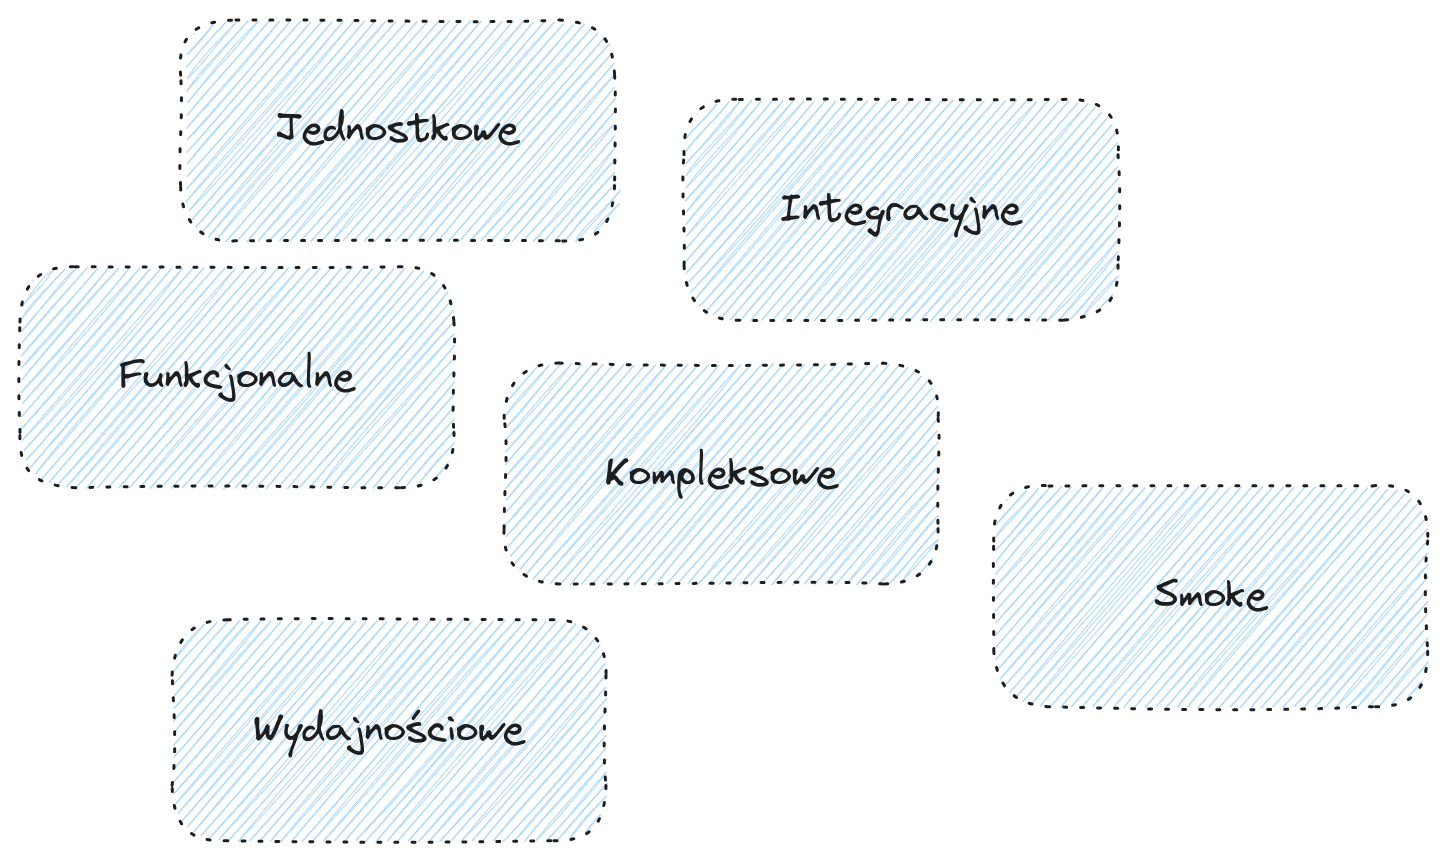
\includegraphics[width=1\linewidth]{rysunki/test-types.png}
	\caption{Rodzaje testów}
	\label{rys:test-types}
\end{figure}
Testy jednostkowe są testami pisanymi na stosunkowo niskim poziomie. Nie jest jednoznaczne czym jest jednostka która jest testowana.
Czasami jest to jedna funkcja, czasem jeden modół.
Wszystko zależy od kontekstu badanego rozwiązania.
Charakteryzują się szybkością działania.
Nie potrzebna jest rozbudowana infrastruktura.
Dzięki temu można je uruchamiać często.

Kolejnymi testami na wyższym poziomie są testy integracyjne.
Badają one współdziałanie różnych modułów ze sobą. 
Do ich uruchomienia potrzebne jest zestawienie kilku modułów ze sobą więc wymagają one zazwyczaj większej infrastruktury niż testy jednostkowe.
Wiąże się to ograniczeniami związanymi ze zwiększonymi kosztami czasowymi oraz często powiązanymi z tym kosztami finansowymi.

Testy funkcjonalne nastawione są na sprawdzenie wymagań biznesowych aplikacji.
Ich złożoność podobna jest do testów integracyjnych.
Dziedziną badania jest sprawdzenie czy kluczowe elementy funkcjonalności są zrealizowane.

Kompleksowe testy badają całą aplikację.
Testy te wymagają postawienia całego systemu w celu jego przetestowania.
Z powodu ich kosztowności zaleca się ograniczenie ilości tych testów do minimalnej liczby.
Posiadanie ich nejlepiej weryfikuje czy badana aplikacja działa.

Testy akceptacyjne weryfikują czy kluczowe wymagania biznesowe są zrealizowane.
Wymagają postawienia całej aplikacji przez co są kosztowne.

Smoke testy są istnym rodzajem testów bardzo łatwym w przeprowadzeniu.
Polegają na pobieżnym przejściu przez dowolny fragment systemu.
Jest to szybka weryfikacja czy podstawowy element systemu działa jak powinien.

Testy wydajnościowe sprawdzają czy w wymaganym obciążeniu aplikacja zachowuje się poprawnie.
Pomagaja znaleźć wąskie gardła systmu i zapobiec przerwie działania w przypadku wzrostu obłsugiwanych użytkowników lub zwiększenia ilości przetważanych danych,

Wraz z wchodzeniem na wyższy poziom testowania koszty testów rosną \cite{testerzyPiramidaTestw}.
Stąd istnieje piramida testów prezentująca zaleźność liczby testów w zależności od rodzajów.
Piramida ta została zaprezentowana na rysunku \ref{rys:test-pyramid}.
\begin{figure}[!hb]
	\centering 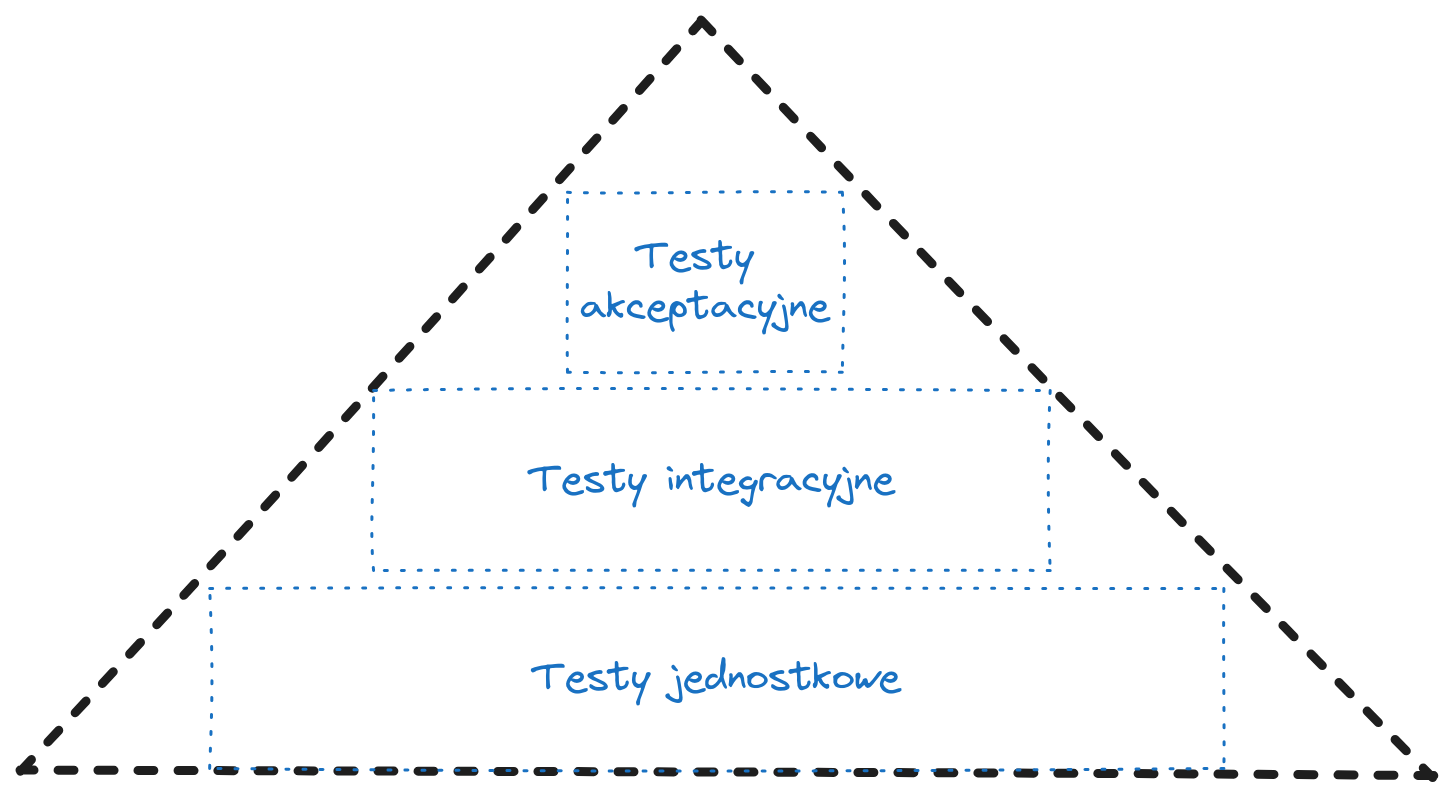
\includegraphics[width=1\linewidth]{rysunki/test-pyramid.png}
	\caption{Piramida testów}
	\label{rys:test-pyramid}
\end{figure}
Testy jednostkowe są na najniższym poziomie piramidy, a więc tego rodzaju testów powinno być najwięcej jako, że testy te są tanie w utrzymaniu.
Na samej górze są testy funkcjonalne, a więc kosztowne w utrzymaniu.
Sposób podziału testów jest umowny więc wszystkie niewymienione rodzaje testów również znajdują się w piramidzie obok najbliższego rodzaju testów.


W niniejszej pracy testy przeprowadzone przynależą do kategorii testów wydajnościowych.
Są to kluczowe testy zapewniające o jednym z istotnych aspektów dobrze działającego oprogramowania.
Ich zadaniem jest identyfikacja obszarów ryzyka zachowania w czasie, wykorzystania zasobów, przepustowości \cite{testerzyTestowanieWydajnoci}.

\begin{figure}[!hb]
	\centering 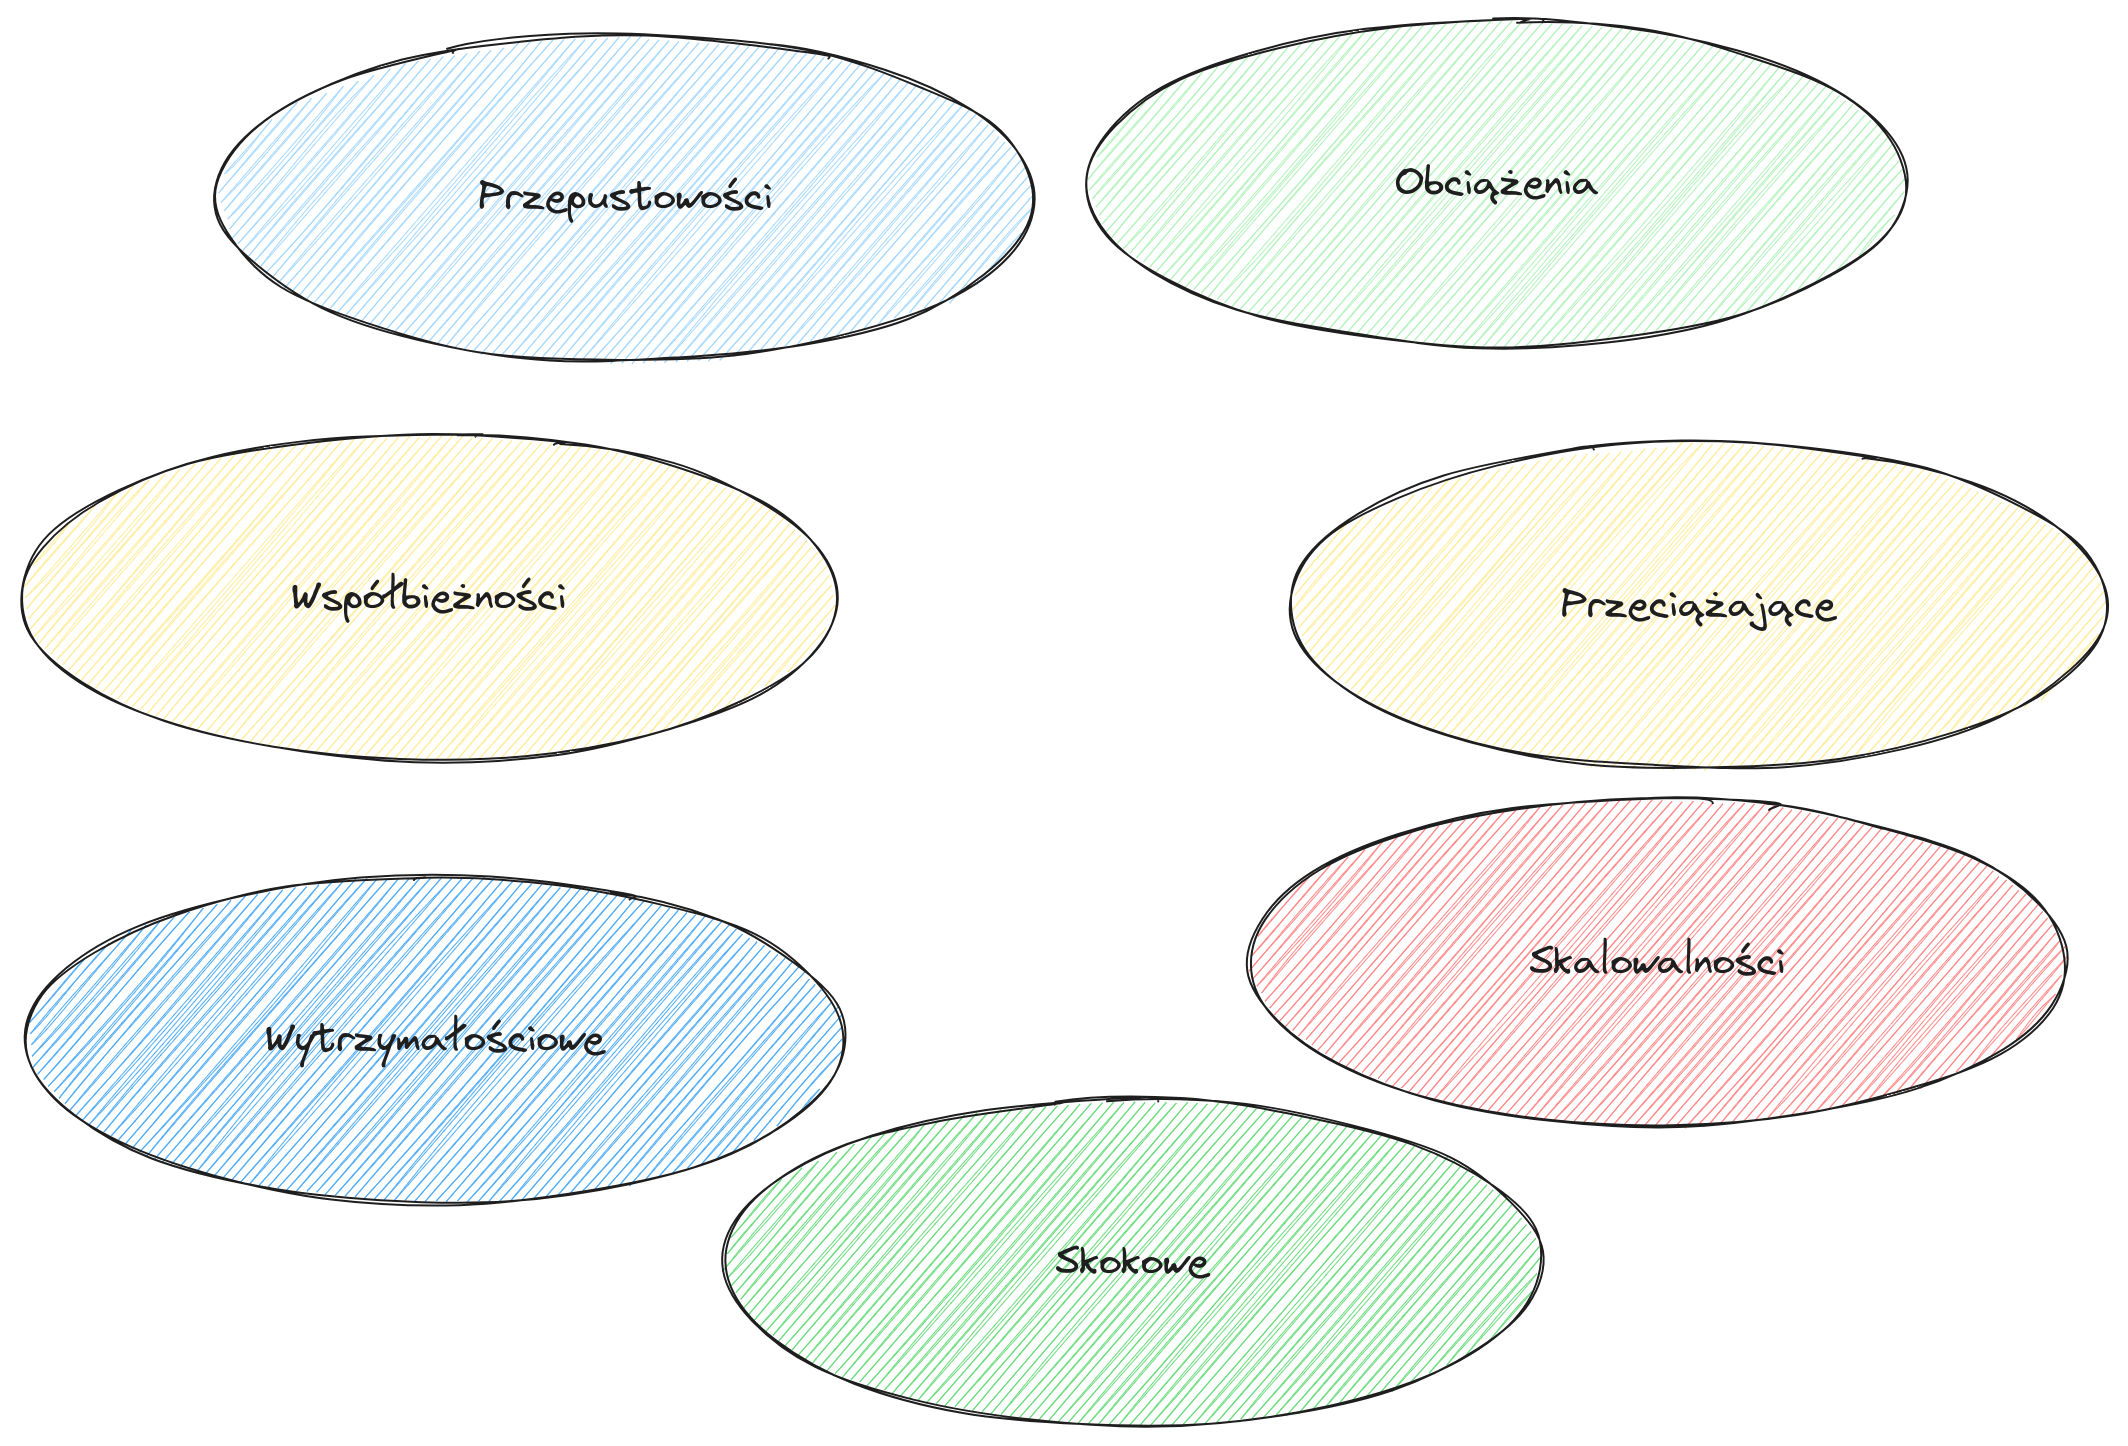
\includegraphics[width=1\linewidth]{rysunki/performance-tests.png}
	\caption{Typy testów wydajnościowych}
	\label{rys:performance-tests}
\end{figure}

Typy testów wydajnościowych zostały zaprezentowane na rysunku \ref{rys:performance-tests}.

Testowanie obciążenia to badanie zdolności systmu do obsługi wzrastającego obciążenia przy realistycznych, przywidywanych ilościach aktorów mających interakcje z systemem.

Testowanie przeciążające to badanie realizowane przy danych przekraczających realistyczne obciążenie. 
Ma ono na celu znalezienie granicy.

Testowanie skalowalności polega na zbadaniu granic funkcjonowania systemu przy zachowaniu większości pierwotnych założeń.
Pozwala ono na monitorowanie i wczesne reagowanie gdy nasz system wraz z rozwojem stopniowo przekracza wytyczone wymagania.

Testowanie skokowe bada reagowanie systemy na nagły, chwilowy wzrost obciążenia.
System powinien być w stanie wrócić no normalnego funkcjonowania, gdy obciążenie wróci do początkowego stanu.

Testowanie wytrzymałościowe skupia się na ocenie działania systemy w dłuższym okresie spracyficznym dla rozwiązania.
Skupia się na drobnych niedokładnościach, które wraz z czasem działania mogą urosnąć do rangi poważnych błędów.
Mogą to być błędy obliczeń związane z zaokrąglaniem lub wycieki pamięci.

Testowanie współbierzności sprawdza czy system działa poprawnie w przypadku przeprowadzania równoległych operacji.
Jestem to zazwyczaj trudny obszar do badania.

Testowanie przepustowości ocenia granice gdy system przestaje działać zgodnie z wymaganiami przy zwiekszonej liczbie aktorów mających interakcje z systemem.

Od innej strony można podzielić na testowanie statyczne oraz dynamiczne.
Testowanie statyczne wiąże się ze sprawdzeniem wymagań, architektury rozwiązania w celu znalezienia wąskiego gardła.
Czasami oznacza to również sprawdzenie używanych algorytmów.
Jest to bardzo ważna weryfikacja, ponieważ może zostać zrobiona w początkowej fazie projektu.
Poprawa problemu we wczesnej fazie zazwyczaj sprawia że jest on zdecydowanie mniej kosztowny.
Testowanie dynamiczne to testy jednostkowe, integracyjne, akceptacyjne, które zazwyczaj powstają wraz z rozwojem systemu.
Ich celem jest zwrócenie uwagi na problem niedostrzeżony w fazie testowania statycznego.
